%\documentclass[aps,twocolumn,floatfix,prl]{revtex4-1}
%\documentclass[letterpaper,10pt,prl,twocolumn,aps]{revtex4-1}
\documentclass[aps,preprint,floatfix,prl]{revtex4-1}
\usepackage{fullpage}
\usepackage{amsmath}
\usepackage{amsfonts}
\usepackage{amssymb}
\usepackage{graphicx}
\usepackage{slashbox}
\usepackage{color}
\usepackage{longtable}
\usepackage{array}
\usepackage{dashrule}

\usepackage{amsmath}

\usepackage{dcolumn}% Align table columns on decimal point

\usepackage{graphicx}% Include figure files
\usepackage{dcolumn}% Align table columns on decimal point
\usepackage{bm}% bold math
\usepackage{ifthen}
\usepackage{amsthm} % Theorem Formatting
\usepackage{amssymb}	% Math symbols such as \mathbb
\usepackage{calrsfs}
\graphicspath{ {images/} }

\newcommand{\ellcap}{{\ell_\text{c}}}
\newcommand{\Fh}{{\boldsymbol{F}_h}}
\newcommand{\Fv}{{\boldsymbol{F}_v}}
\newcommand{\Tv}{{\boldsymbol{T}}}
\newcommand{\bn}{{\boldsymbol{n}}}
\newcommand{\bt}{{\boldsymbol{t}}}
\newcommand{\bz}{{\boldsymbol{z}}}
\newcommand{\bx}{{\boldsymbol{x}}}
\newcommand{\by}{{\boldsymbol{y}}}
\newcommand{\bT}{{\boldsymbol{T}}}
\newcommand{\bu}{\mathbf{u}}
\newcommand{\grad}{\mathbf{\nabla}}
\newcommand{\del}{\partial}

\begin{document}

\title{Waving and swaying}
\author{Ravi Singh}
\affiliation{Brown University, Providence RI 02912 USA}
\author{L. Mahadevan}
\affiliation{Harvard University, Cambridge MA 02138 USA}
\author{Mahesh Bandi\footnote{work performed while visiting Brown University}}
\affiliation{Okinawa Institute of Science and Technology, Okinawa, Japan}
\author{Amala Mahadevan}
\affiliation{Woods Hold Institute of Oceanography, Woods Hole MA USA}
\author{Shreyas Mandre}
\affiliation{Brown University, Providence RI 02912 USA}

\begin{abstract}
The spontaneous waving of marine grass is thought to be due to a Kelvin-Helmholtz instability resulting from an inflection point in the flow profile. 
We find that this inflection point is located inside the grass canopy, and the drag from the grass blades damps out the Kelvin Helmholtz instability, 
normally observed in a free shear layer. We also show that the wavelength of coherent vortices scales with the unvegetated water depth, and not with 
the shear layer thickness as predicted by a theory based on Kelvin-Helmholtz instability. Based on these results, we propose a mechanism for waving 
marine grass based on the shear instability of the flow above the canopy.
\end{abstract}
\maketitle

\section{Introduction}
Sea grasses exhibit rich set of dynamics due to their interaction with the flow of water and can considerably affect surrounding hydrodynamic conditions.
%Rich set of dynamics are exhibited by sea grasses due to their interaction with water flow which can considerably affect the hydrodynamic conditions near the 
%grass.
Resulting changes in hydrodynamic conditions relative to unobstructed flow can influence number of environmental variables and processes such as 
transport of sediments, contaminants, dissolved oxygen, plant growth and biomass production etc. 
%Driven by such applications number of scientific work regarding flow over canopies has been done over 
%last three decades. One of main development is recognition that major contribution to canopy turbulence arises from coherent eddies
%of canopy scales.\newline
The response of flexible grass canopies to steady current in form of large amplitude coherent oscillations known as mo-nami (Ackerman and Okubo, 1993) plays a central role
in the recruitment of microscopic marine organism such as blue mussel larvae. The hydrodynamic mechanism underlying monami is the focus of this paper. 
%Among many dynamics shown by flexible grasses due to their interaction with water flow, their response to steady current in form of large amplitude coherent oscillations known as
%mo-nami (Ackerman and Okubo 1993) is focus of this paper. 
Similar phenomenon of large amplitude coherent oscillation of canopy in wind known as ho-nami (Inoue 1955) have also been observed.
% Experimental observations (Grizzle 1996) have shown that monami is observed when mean flow speed exceed a certain threshold value. 
\newline
Although atmosphere flow through terrestrial canopies seems similar to aquatic flow through vegetation, atmospheric flows are essentially unbounded vertically. Another major
difference between atmospheric flow and aquatic flow is the considerable difference of stiffness of canopies, terrestrial canopies tends to be much more rigid than marine canopies.
\newline   
The previous explanation of mo-nami invokes the existence of strong shear near the top of the canopy (Ghisalberti 2002, Raupach 1996) due to
different amounts of drag experienced by fluid in and above the canopy. Existence of strong shear is manifested by
the presence of an inflection point in the mean velocity profile near the top of the canopy.
% In addition pattern of coherent eddies propagating downstream 
%along have also been observed.
%A crucial feature of a velocity inflection is that it induces a hydrodynamic instability
%process which sets the pattern of coherent eddies propagating over terrestrial and submerged canopies. In response to coherent eddies canopies
%may exhibit synchronous large-amplitude waving (termed as monami in aquatic setting by Ackerman and Okubo[1993], and honami by Inoue (1955) in terrestrial setting). 
%Monami (Honami) can be observed when flow velocity is above certain threshold value, which can depends on flow depth, elasticity of canopy material
%etc.
%\newline
%Following the work of Raupach (1996) on terrestrial canopies, 
Existing explanation of monami have been done under assumption that the a pattern of coherent eddies are excited by hydrodynamic instability of shear layer
similar to that of free shear flow known as Kelvin-Helmholtz instability. Influence of these coherent eddies over sea grasses are exhibited by their large amplitude synchronous 
oscillations.
%Sea grasses exhibit large amplitude wave like motion in response to these eddies propagating downstream.
%are exhibited in form of large amplitude oscillations knows as mo-nami.
\newline
While shear layer model successfully predict frequency of mo-nami for number of experimental observations,
several aspect of existing theory remain unexplained. First, the proposed hydrodynamic instability of shear layer produced due to drag of 
grass does not take into account influence of drag due to grasses itself. 
%the proposed hydrodynamic instability mechanism of shear layer layer does not take into account presence of grass whereas existence of 
%shear layer is due to drag provided by vegetation. 
Second, classical free shear flow is known to be unstable above a very small Reynolds number $\leq 10 $. On the contrary observed critical Reynolds number (Grizzle 1996) for monami is much
higher $\sim 1000$
%(Grizzle,1996) shows that an event of mo-nami is not observed until flow speed exceed a certain threshold value. Although atmospheric flow through terrestrial canopy seems similar to 
%aquatic flow through vegetation, atmospheric flow is essentially unbounded, due to these difference of vertical extent of flow in two cases a mechanism similar to 
%terrestrial case might not be adequate for aquatic scenario.
%might not hold  
%was produced due to drag caused by presence vegetation. 
%Second, shear layer instability mechanism does not predict any threshold for monami, hence it fails to explain
%observations where monami is observed when mean flow speed is above certain value. While atmospheric flow through terrestrial vegetation seems similar to aquatic flow through marine grass, 
%atmospheric flow is unbounded in vertical direction.
% but aquatic flow is not so its not obvious that similar mechanism will hold in aquatic case too (2) The proposed hydrodynamic instability mechanism of shear layer produced 
%by presence of grass does not take into account the presence of grass itself (3) It does not predict any threshold condition for waving to happen 
\newline 
 In this paper we extend the idea of Raupach et.al via incorporating drag due to presence of vegetation. Our calculation of linear stability analysis of flow in presence of grasses 
shows that drag from the grass blades damps out the Kelvin Helmholtz instability. We also show instead that mo-nami is caused by instability 
of fluid flow above vegetation coupled with the flow through canopy. We further show that inclusion of drag due to grass predicts a threshold condition for waving where threshold is
characterized by Reynolds number. We confirm our analysis by comparing prediction from theory with field and experimental observations.  
%In this paper we propose a coupled fluid-canopy model to study dynamics of flexible canopy and flow field. Canopies are represented by a continuous 
%medium which is coupled to flow field via a drag term. We did linear stability analysis of flow without ignoring presence of grass via solving 
%a generalized orr-sommerfield equation with presence of grass. Our calculation predicts threshold a threshold criteria for waving which is characterized by Reynolds number.
%We further show that for flexible marine grass monami is caused by instability of flow above the grass rather than by shear layer. We confirm our analysis by comparing 
%prediction from theory with existing data

\section{The model}
We use a mean field model for the coupling between the flow and the canopy. Assuming strong oscillation in fluid flow is caused by instability of flow
composed of regions experiencing higher drag with in grass and less outside while monami being response of flexible grass to oscillations of fluid flow. We expect stiffness 
of grass to play minor role in development of flow instability. We approximate grasses with stiff cylindrical rod of diameter $d$ and height $h$ with number density $N/m^2$. 
Drag force exerted by the grass is approximated via a continuous body force $\mathbf{f}=-N\mathbf{f_d}$ in the fluid momentum balance as
%We propose a fully coupled model in order to comprehend dynamics of canopy and fluid flow, drag force excerted by grasses is
%taken as an additional body force in momentum equation of fluid. We approximate presence of grass via continuous field whose shape at any location is approximated as averaged 
%shape of grass at that location which can be obtained by assuming grass to be in quasi-equilibrium at any moment.
% and solving force balance and momentum balance for grass  
\begin{equation}
\rho \left(\bu_{t}+\bu.\grad\bu \right) = -\grad P+\mu\grad^{2}\bu +\mathbf{f}+\rho\mathbf{g}
\end{equation}
%\begin{equation}
% \mathbf{f}=-N\mathbf{f_{d}}
%\end{equation}
where $\mathbf{f_{d}}$ is drag force per unit length of grass, $\rho$ the fluid density, $\mathbf{u}$ the velocity, $P$ the pressure, $\mu$ the viscosity and $\mathbf{g}$
the acceleration due to gravity. Drag force itself is modeled as $\mathbf{f_{d}}=C_N \rho\bu_{N}^{2}d\hat{n}+C_{T}\rho\bu_{T}^{2}d\hat{t}$ where 
$C_{N}$ and $C_{T}$ are normal and tangential drag coefficients respectively which are set to zero outside the grass; $\bu_{T}$, $\bu_{N}$ are velocity vector along and
normal to grass while $\hat{t},\hat{n}$ being unit vector along and normal to grass. We expect $C_T \ll C_N$ and take $C_T=0$ for rest of analysis. We further expect $C_N$ to
not change along the height of the grass and take $C_N$ to be constant for further analysis. 
%\begin{equation}
% \mathbf{f_{d}}=C_N \rho\bu_{N}^{2}d\hat{n}+C_{T}\rho\bu_{T}^{2}d\hat{t}
%\end{equation}\


%\begin{equation}
%\begin{split}
% \frac{\del}{\del s}\left(T\hat{t}+N\hat{n}\right) & +\mathbf{f_{d}}+\mathbf{f_{buoy}} = 0\\
% \frac{\del M}{\del s}&-N = 0\\
% M &= B\kappa
%\end{split}

%\end{equation}
%where $C_{N}$ and $C_{T}$ are normal and tangential drag coefficients respectively; $\bu_{T}$, $\bu_{N}$ are velocity vector along and normal to grass.
  
%\begin{center}
%\begin{figure}[ht]
%\begin{minipage}[b]{5cm}
%\begin{center}
%\centering
% 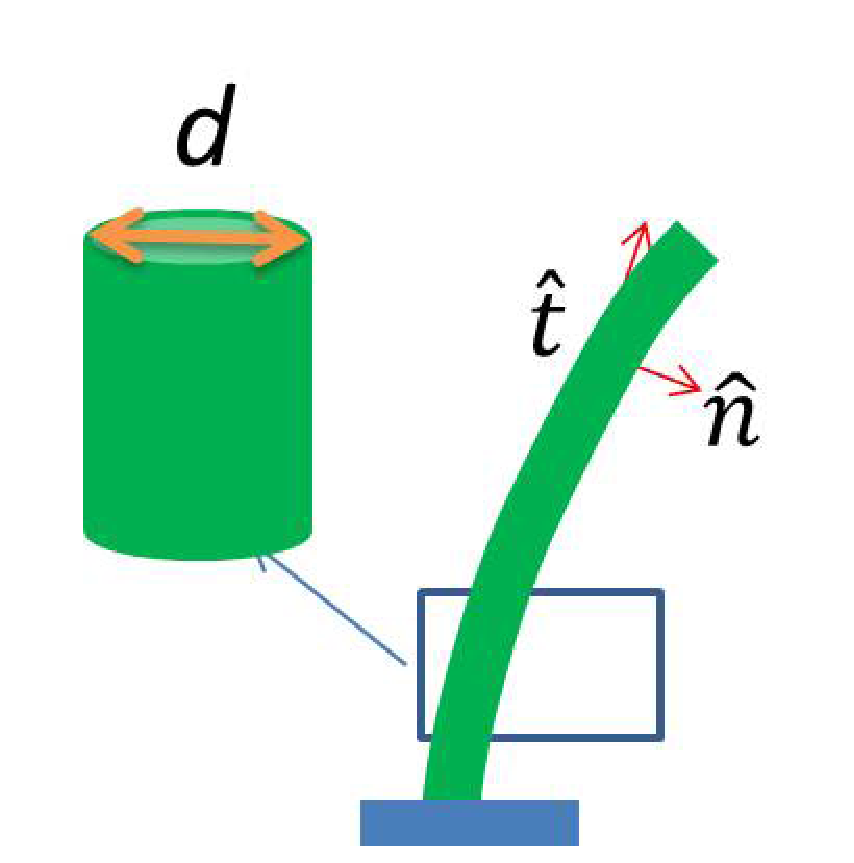
\includegraphics[width=4.0cm,height=4.0cm]{Grass_orientation}
%\caption{Typical grass orientation}
%\end{minipage}
%\hspace{1.0cm}
%\begin{minipage}[b]{5cm}
%\centering
% 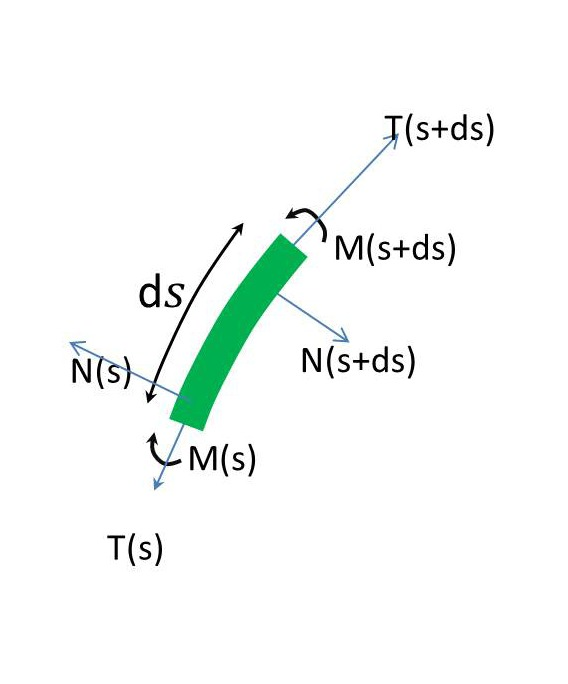
\includegraphics[width=5.0cm,height=5.5cm]{Grass_orientation2} 
%\caption{Forces and moment on a section of grass}
%\end{minipage}
%\end{figure}
%\end{center}
%For flexible grass whose bending stiffness is really low, we assume that monami/honami is response to oscillations in flow velocity of fluid. In that case we can safely ignore
%set of equation(3).
\section{Stability Analysis}
In order to understand frequency and wavelength associated with passage of dominant eddies over grass which are manifestation of hydrodynamic instability associated with mean flow, 
we investigate stability of base flow profile which is obtained by solving steady state solution of equation(1). Considering small perturbations $u, v, p$  associated 
with base profile $U$ and $P$ respectively, momentum and mass balance equation expanded in 1st order of perturbed variable yields.
\begin{equation}
\begin{split}
 \frac{\del u}{\del t}+U\frac{\del u}{\del x}+v\frac{\del U}{\del y} &= -\frac{1}{\rho}\frac{\del p}{\del x}+\frac{\mu}{\rho}(u_{xx}+u_{yy})-2C_{N}dN_{g}Uu\\
 \frac{\del v}{\del  t}+ U\frac{\del v}{\del x} &= -\frac{1}{\rho}\frac{\del p}{\del y}+\frac{\mu}{\rho}(v_{xx}+v_{yy})\\
 \nabla\cdot \bu &= 0
\end{split}
\end{equation}
%In most of recent work on honami/monami base profile have been approximated to a plane mixing layer profile having inflection point near top of canopy, It is also argued that 
%It is instability associated with inflection of mean velocity which is responsible for coherent eddies traveling on top of canopies. In our calculation we get base velocity
%profile by hydrodynamic balance between pressure, drag and diffusive force which also results in a velocity profile with inflection point near top of canopy with additional property 
%of having been produced through equation of motion itself.\newline
%We performed stability analysis on two different kind of base flow namely (1) flow driven by constant pressure gradient between two parallel plate (2) constant pressure gradient driven 
%flow with zero shear at top. We use following scaling to non-dimensionlize equation of motion
Where drag coeffient $C_N$ is set zero out side vagetation. Using height $H$ of fluid column and associated advection time H/$U_{0}$, we use following scalaing to non-dimensinlize equation 
of motion
   \[ u = U_{0}\bar{u},\hspace{1cm} y = (H/2)\bar{y}, \hspace{1cm} \text{with}\hspace{2mm} U_{0}=\frac{(dP/dx)H^2}{4\mu} \]
With these scaling along with the use of stream function $\psi$ with $u = \psi_{y}, v= -\psi_x$, equations can be simplified into a single equation.
\begin{equation}
\begin{split}
 R_{e}\left[\psi_{yyt}+\psi_{xxt}+U\left(\psi_{xyy}+\psi_{xxx}\right)-U_{yy}\psi_{x} \right] &=\left[\psi_{yyxx}+\psi_{yyyy}+\psi_{xxxx}+\psi_{xxyy} \right]\\
& + 2D_{drag}U\psi_{y}\delta(y-h)\\
& - 2D_{drag}U_{y}\psi_{y} -2D_{drag}U\psi_{yy}
\end{split}
\end{equation}
where $R_{e}= \frac{\rho U_0 H}{2\mu}$ is Reynolds number and $\bar{N_g} = C_N d N_g H/2$ is non-dimensional grass number density and  $D_{drag} = R_{e}\bar{N_{g}}$ is non-dimensional.
Seeking wave solution in form of $\left(u,v,\psi \right)= \left(\hat u, \hat v, \hat\phi \right)e^{ikx+\sigma}$, we get generalized orr-sommerfield equation 
which is an eigenvalue problem whose solution provides frequency and wavelength of eddies traveling over canopy.
\begin{equation}
\begin{split}
\sigma \left(D^2-k^2\phi \right) &= \frac{1}{R_{e}}\left[D^4\phi -2k^{2}D^2\phi +k^{4}\phi \right]\\
				  & +ikU_{yy}\phi-ikU\left(D^2\phi-k^2\phi \right)\\
 & -\frac{2D_{drag}}{R_{e}}U_{y}\phi_{y}-\frac{2D_{drag}}{R_{e}}U\phi_{yy}+\frac{2D_{drag}}{R_{e}}U\phi_{y}\delta(y-h)
\end{split}
\end{equation}
Critical Reynolds number above which we get growing solution of perturbation, as a function of grass number density for different grass height shows following characteristics 
  \begin{figure}[htb!]
  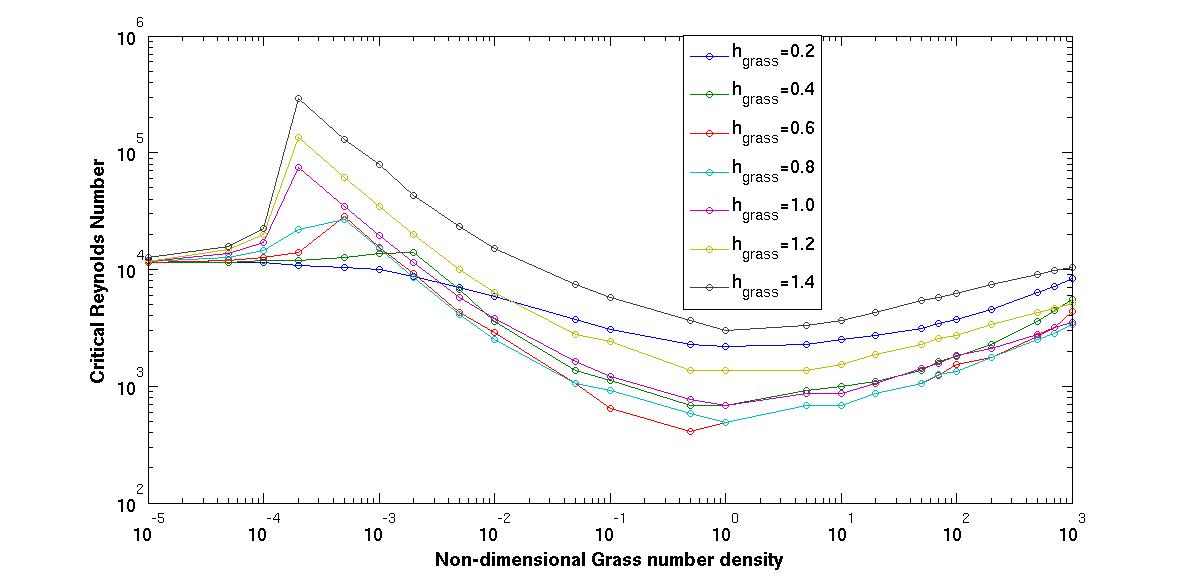
\includegraphics[scale=0.35]{Instability2}
\caption{Critical Reynolds number with flow between parallel plate for different grass height as a function of grass number density}
\end{figure}

\begin{figure}[htb!]
  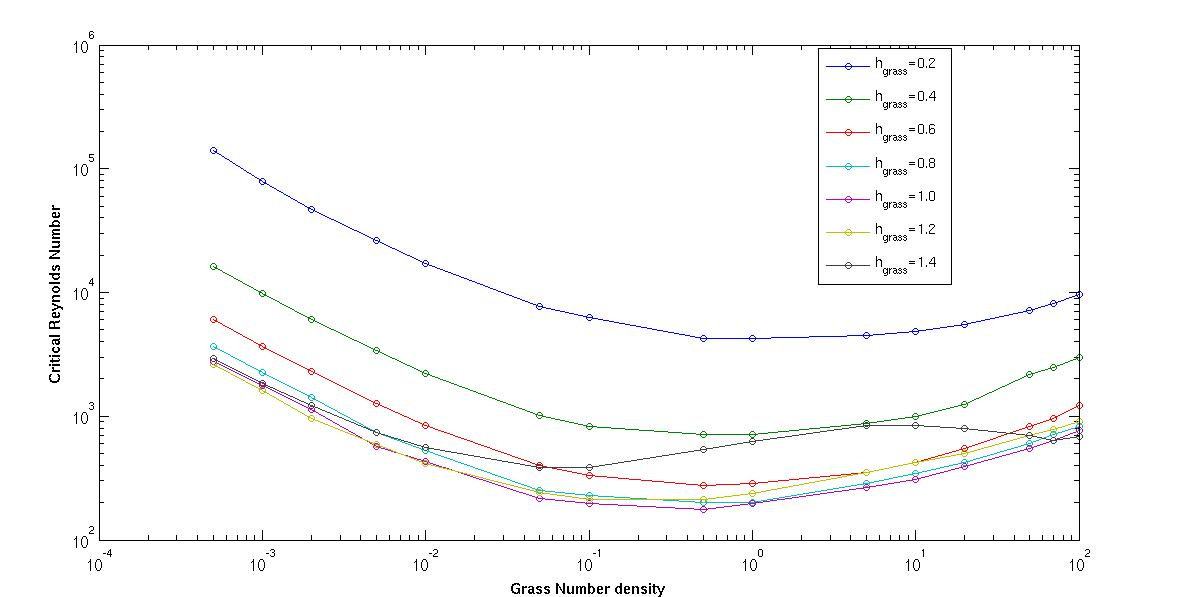
\includegraphics[scale=0.35]{Instability1_free.jpg}
\caption{Critical Reynolds number with no shear stress at top for different grass height as a function of grass number density}
\end{figure}

\end{document}
